 \documentclass{/home/janmebows/Documents/LatexTemplates/myassignment}


\title{Modelling With ODEs}

\begin{document}

\maketitle

\section{Introduction}
\subsection{Prelim}
This course concerns DEs with only one independent variable, and varying numbers of dependent variables. We will consider scalar ODEs with a single dependent variable, vector ODEs, and equivalently, systems of ODEs having vector (or multiple) dependent variables.


Two types of problems:
\begin{itemize}
    \item Dynamics (temporal problems): Independent variable is time. Unknown (dependent) function will be $\vec{u}(t)$. We will need an Initial condition, e.g. at $t=t_0$ $\vec u(t_0) = \vec u_0$
    \[\text{ODE} + \text{ initial value } = \text{ IVP}\]
    \item Spatial problems (BVPs): Independent variable is space, and unknown dependent function will be $\vec u(x)$. We will need two boundary conditions, e.g. a value at $x=a$ giving  $\vec u(a) = \vec u_a$ and at $x=b$ giving $u(b) = u_b$
    \[\text{ODE} + \text{ Boundary Values } = \text{ BVP}\]
\end{itemize}
We can also have derivative boundary/initial conditions

\subsection{Dynamics, Modelling and Computation}
\subsubsection{Modelling}
Deriving solutions for real world problems, given a worded problem and associated ICs or BCs. Use to predict and understand behaviours and complex interactions.
\ex{Simple Pendulum}
Let $\theta(t)$ be the angle away from directly down, $l$ be the length of the pendulum, $m$ be the mass of the pendulum, and $g$ be the force due to gravity.\\
Assumptions:\\
Mass $m$ is much greater than the mass of the string (neglect mass of string) $m >> m_{string}$. Gravity is the only force acting.\\
Independent variable: $t$. Lastly assume $m,g,l$ are constant.\\
Dependent variable $\theta(t)$.\\
Initial condition: $\theta(0) = \theta_0$\\
Mechanics problem: resolve motion of mass into the normal of the mass, and the tangent to the string. Note there is no motion in the normal. So we only consider the tangent. We find that these are directly related to $\theta(t)$. \\
Apply Newtons second law
\begin{align*}
    F&=ma\\
    F_{norm}&= ma = 0*m = 0\\
    F_{tan}&= ma=ml\ddn{\theta}{t}{2}\\
    F_{tan} &=-mg \sin(\theta)\\
    -mg\sin(\theta) &= ml\ddn{\theta}{t}{2}\\
    -g\sin(\theta) &= l \ddn{\theta}{t}{2}\\
    \ddn{\theta}{t}{2} + \frac{g}{l} \sin(\theta)&= 0
\end{align*}
The $F_{tan}$ lines are found by resolving forces and basic trig
Initial Condition: assume the mass is released at $\theta(0) = \theta_0$ which also means $\frac{d\theta}{dt}|_{t=0} = 0$ 
For this problem the parameters were mass, the length of the string, gravity and the initial angle we release the string at. However we do find that the mass cancels out.

While this could be solved exactly (even though its non linear) by double integrating $\sin(\theta)$ that would go against the philosophy of the course...\\
Time to approximate. Lets use forward difference approximation (Euler's method).
\[\frac{df}{dt} \approx \frac{f(t+h) - f(t)}{h}\]
Where $h$ is a small perturbation.

Turn the 2nd order scalar ODE into a first order system of
\begin{align*}
    x(t) &= \theta(t)\\
    y(t) &= \frac{d\theta}{dt} = \frac{dx}{dt}
\end{align*}
The system becomes:
\[\frac{dx}{dt} = y , \quad \frac{dy}{dt} = -\frac{g}{l}\sin(x)\]
With the initial conditions 
\[x(0) = x_0 =\theta_0, \quad y(0) = 0\]
Using the forward difference approximation to the system:
\begin{align*}
    \frac{x(t+h) - x(t)}{h} &= y(t)\\
    \implies x(t+h) &= x(t) +hy(t) \\
    \frac{y(t+h)-y(t)}{h} &= \frac{-g}{l} \sin(x(t))\\
    \implies y(t+h) &= y(t)+ \frac{-gh}{l} \sin(x(t))\\
\end{align*}
So what we are saying is the values of $x$ and $y$ at time step $h$ into the future, it is equal to a function of the values at the present. These are known as update formulae 
Start with $t=t_0=0$:
\[(x_0,y_0) = (\theta_0,0)\]
Then increment $t$ to $t+h$.
\[(x_1,y_1) = \left(x(t) + hy(t),y(t)+ \frac{-gh}{l} \sin(x(t)\right)= \left(x_0, \frac{-gh}{l} \sin(x_0)\right)\]
This method is known as \textbf{time stepping}.\\
We could have alternatively used finite differences (PDEs) to approximate the second order derivative, and then we wouldn't have had to convert the ODE into a system.\\
Alternative: assume $\theta$ is small, then use 
\[\sin\theta \approx \theta\]
The ODE becomes linear:
\[\frac{d^2\theta}{dt^2} \approx- \frac{g}{l} \theta\]
Which is very easy to solve:
\[\theta = \theta_0 \cos(\sqrt{g/l} t)\]
Of course this is ONLY valid when $\theta$ is small (so $\theta_0$ must be small).

Note that there are some very trivial solutions to this problem. $\theta(t) = 0$ and when $\theta(t) = \pi$, since $\sin(\theta) = 0$ if $\theta=0,\pi$. I.e. when $\theta$ is vertical  
The fundamental difference between these two states is $\theta=\pi$ is \textbf{unstable}. By shifting $\theta$ by some $\delta$ such that $\theta = \pi \pm \delta$ we find it will drastically change the state.

\subsubsection{Dynamics}
Whoops i think this started earlier...
\subsubsection{Computation}
Ideally we would have exact solutions to ODEs (no errors and more useful as analytic). Unfortunately most ODEs cannot be solved exactly, so we use approximations (yay practical asymptotics). We find a trade-off between error and computational time. Remember that the models we use are approximations of the real world anyway (we might miss factors or something).
Simpler models are more likely to be solvable, but they are less likely to be realistic and applicable.



\subsubsection{Analysis}
This is the most important part. Converting the problem into a format which is useful to both mathematicians and non-mathematicians. I.e. This analysis is more reflecting what sort of real behaviour we think. We want to interpret what the model predicts for the initial problem. 




\section{One-Dimensional autonomous ODE models}
We want to be able to use \textbf{phase line analysis} to determine long-term behaviour of solutions, to be able to identify \textbf{fixed points} and determine their \textbf{stability}. The goal is to be able to apply suitable \textbf{non-dimensionalisations} of IVPs and to be able to identify and classify \textbf{bifurcations} in solutions as parameters are varied.
\subsection{Autonomous Scalar Equations}
A general first order scalar ODE has form
\[\frac{dx}{dt} = f(x(t),t)\]
If $f$ does not explicitly on $t$. I.e:
\[\frac{dx}{dt} = f(x)\]
Then the equation is \textit{autonomous} as it only implicitly depends on time (through $x(t)$). For this section we will only consider autonomous scalar ODEs.






\subsection{Fixed Points, phase line analysis, and stability criteria}
We are looking to consider the long term behaviour of these autonomous ODEs.
\subsubsection{Fixed Point}
For the first order, one dimensional, autonomous ODE:
\[\frac{dx}{dt} = f(x(t))\]
The \textit{fixed points}, \textit{steady states}, or \textit{equilibria} of the ODE are the values of $x = x^*$ such that:
\[\frac{dx}{dt}\pipe_{x^*} = 0, \quad \Leftrightarrow \quad f(x^*)=0 \]

Example: Logistic equation
\[\frac{dx}{dt} = f(x) = rx(1-\frac{x}{k})\]
$x(t)$ is the population, $r$ is the growth rate, and $k$ is the carrying capacity. We have 2 parameters ($r,k$).

Of course the assumption that $x(t)$ is discrete or alternatively that it is a proportion. If we consider it as a proportion then we assume that it is very large (this is where non-dimensionalisaion comes in). This is the continuum approximation.

Looking for fixed points gives:
\[x^* = 0, \quad x^* = k\]

\subsubsection{Phase Line Analysis}
If we take a perturbation for $x^*$ to either side, what do we expect to happen?
\begin{enumerate}
    \item if $\frac{dx}{dt} > 0$ then the population will increase. 
    \item if $\frac{dx}{dt} < 0$ then the population will decrease.
    \item if $\frac{dx}{dt} = 0$ then the population will stay where it is.
\end{enumerate} 
Basically graphically if the arrows point towards the fixed point then it is stable, if they move away then it is unstable.

This is phase line analysis.



\subsubsection{Stability}

It shows that $x^*=0$ is an unstable point as a perturbation will shift the system away from $0$, and $x^*=k$ is stable as we would expect it to return to $x^*=k$

More rigorously:
If we shift $x^*$ by $\delta x \ll 1$ then (by using taylor's theorem)
\begin{align*}
\frac{dx}{dt}\pipe_{x=x^*+\delta x} &= f(x^* + \delta x)\\
&= f(x^*) + \delta x f'(x^*) + \hdots\\
&= \delta x f'(x^*) + \hdots
\end{align*}
The possibilities are:
\begin{enumerate}
    \item $f'(x) < 0 $: 
    \[\implies \begin{cases}\delta x f'(x^*) < 0 \quad \delta x < 0, \quad x\text{ decreasing for } \delta x > 0\\
    \delta x f'(x^*) > 0\quad \delta x < 0, \quad x \text{ increasing for } \delta x <0\end{cases}\]
    I.e. $x$ returns to the steady state, and thus it is \textbf{stable}.
    \item $f'(x) > 0 $: 
    \[\implies \begin{cases}x \text{ increasing for } \delta x <0\\
    x \text{ decreasing for } \delta x > 0\end{cases}\]
    I.e. $x$ shifts away from the steady state. Therefore the steady state $x$ is an \textbf{unstable} point
    \item $f'(x) = 0 $: We then need to consider the next term in the series: $\frac12 \delta x^2 f''(x^*)$.
    \[\implies \begin{cases}x^* \text{ is stable if } f''(x^*) < 0\\
    x^* \text{ is unstable if } f''(x^*) > 0 \\
    x^* \text{ is semi-stable if } f'(x) = 0, \ \text{ and }x^* \text{ is a turning point}
    \end{cases}\]
    Semi-stable points are essentially considered unstable.
\end{enumerate}
Alternatively we can check for these graphically:
If there is a negative slope at $x^*$ then it is stable, positive slope it is stable and then $0$ slope then it is semi-stable.

Example:
\[\frac{dx}{dt} = x^2\]
The equilibria are $x=0, x=0$.
We get
\[f'(x) = 2x \implies f'(x^*)= 0\]
\[f''(x) = 2 \implies f''(x^*) = 2\]
So we find that $x^*$ is semi-stable.

Another example:
\[\frac{dx}{dt} = x(1-x)(2-x)\]
Fixed points at $x^*=0,1,2$
\[f'(x) = 3x^2 - 6x + 2\]
\[f'(x) = \begin{cases}2 & x=0\\ -1 & x=1\\2&x=2\end{cases}\]
So $x=0$ is unstable, $x=1$ is stable, and $x=2$ is unstable.

We would expect alternating between stable and unstable (unless it happens at a turning point [semi-stable point]).



\subsection{Non Dimensionalisation}
Consider the fishing example (2.5).
\[\frac{dN}{dt} = BN - DN^2 - g(N), \quad N(0) = N_0\]

Where $N$ is the number of fish, $B$ is a birth rate, $D$ is the death rate, and $g(N)$ is the yield from fishing. Note that this is the logistic model with an extra term (the yield term). We have 3 visible parameters ($B,D,N_0$)Note that there could be more parameters in $g(N)$.
We can reduce the number of parameters via non-dimensionalisation.
If we define dimensionless terms:
\[ \hat{t}, \quad \hat{N}(\hat{t}) \]
Such that
\[t = t_c \hat{t}, \quad N = N_c \hat{N}\]
Where $N_c$ and $t_c$ are the (characteristic) scales for the fish population and time respectively.
We want to choose $N_c$ and $t_c$ to reduce the number of parameters.
\[N_c = K = \frac{B}{D}, \quad t_c = \frac1B\]
Gives:
\[\frac{d\hat{N}}{d\hat{t}} = \hat{N}(1-\hat{N}) - \hat{g}(\hat{N}), \quad \hat{N}(0) = \hat{N}_0 = \frac{N_0}{N_c}\]
Note we now have parameters $\hat{N}_0$ and any in $\hat{g}$ which is less than we had originally.

To find $N_c,t_c$:
\begin{enumerate}
    \item Substitute $N=N_c\hat{N}$ and $t=t_c\hat{t}$ into the dimensional ode.\\
    LHS:
    Note that $\frac{d\hat{t}}{dt} = \frac1{t_c}$
    \begin{align*}
        \frac{dN}{dt} &= \frac{d}{dt}( N_c\hat{N})\\
        &= \frac{d\hat{t}}{dt} \frac{d}{d\hat{t}} (N_c\hat{N})\\
        &= \frac{N_c}{t_c} \frac{d\hat{N}}{d\hat{t}}\\
    \end{align*}
    RHS:
    \begin{align*}
        BN - DN^2 - g(N) = B N_c \hat{N} - D N_c^2 \hat{N}^2 - g(N)
    \end{align*}
    Combine
    \begin{align*}
        \frac{N_c}{t_c} \frac{d\hat{N}}{d\hat{t}}&=  B N_c \hat{N} - D N_c^2 \hat{N}^2 - g(N)\\
        \frac{d\hat{N}}{d\hat{t}}&=  Bt_c\hat{N} - D N_c t_c \hat{N}^2 - \frac{t_c}{N_c}g(N)\\
        \frac{d\hat{N}}{dt} &= B t_c \hat{N} (1 - \frac{N_c}{K} \hat{N}) - \hat{g}(\hat{N})
    \end{align*}
    Where $k=\frac{B}{D}$ and $\hat{g}(N) = \frac{t_c}{N_c} g(N)$
    \item Choose the scales to simplify the ODE.\\
    Want to simplify the $Bt_c$ and $\frac{N_c}{K}$ terms.
    So 
    \[t_c = \frac1B,\quad N_c = K = \frac{B}{D}\]
    Giving
    \[\frac{d\hat{N}}{dt} = \hat{N} (1-\hat{N}) - \hat{g}(\hat{N}) \]
\end{enumerate}

If we now suppose $g(N) = Y = const$
Then
\[\hat{g}(\hat{N}) = \frac{t_c}{N_c} Y = \frac1B \frac DB = \frac{YD}{B^2} = y\]
Which is still constant.


This reduces the number of parameters to $2$ since we have an initial condition and a parameter $y$.

Once we have solved the non-dimensional IVP, to get the dimensional answer out, we just convert back to the dimensional terms:
\[N = N_c \hat{N},\quad t=t_c \hat{t}\]
But you must know the parameters within $N_c$ and $t_c$ to give this answer back.

So the reasons we non-dimensionalise:
\begin{enumerate}
    \item Reduce the number of parameters
    \item Improves analysis
    \begin{enumerate}
        \item Easier to see the type of equation (and solve it)
        \item Easier to see how it changes with respect to parameters when there are less (especially if solving numerically)
        \item Results are more compact
        \item Solutions for one system can be applied to other systems with the same scaled equation but different parameters)
    \end{enumerate}
    \item It helps 'experimental validation' using a smaller-scale version. We can see how to choose parameters for an experiment without changing the behaviour or the model (good for experimental validation)
    \item We can see the relative importance of the different terms in the equations - even if we can't reduce the number of parameters!
\end{enumerate}

This next bit isn't examinable\\
Point $4$ in that list requires some care... 
Basically we can't use asymptotic relations in certain regions of the problem.


Its worth paying attention to small and large terms like in practical asymptotics and using that to approximate solutions.


\subsection{Bifurcations}
A bifurcation is a qualitative change in the behaviour of the system due to the effect of varying a parameter.

A bifurcation point is a point in which a parameter to the ODE can create or destroy fixed points depending on its value. We do not consider the initial condition to relate to bifurcation points.


Definition:\\
For the ODE
\[\dd xt = f(x:\mu)\]
Where $\mu$ is a scalar parameter, $\bar{x}$ is a bifurcation point, with bifurcation value $\bar{\mu}$ 
if
\[f(\bar{x}:\bar{\mu}) = 0,\quad \dd fx (\bar{x}:\bar{\mu})= 0\]
I.e. a fixed point, with derivative equal to zero.

So if we consider
\[f(\hat{N} : y) = \hat{N}(1-\hat{N}) - y\]
This is $0$ for 
\[\hat{N} = \frac{-1\pm \sqrt{1-4y}}{2}\]

\begin{align*}
    \dd f{\hat{N}} &= 1-2\hat{N}\\
    &=1 - (1\pm \sqrt{1-4y})\\
    &= \mp \sqrt{1-4y}\\
    \implies \bar{y}&=\frac14
\end{align*}
And $\bar{\hat{N}} = 1/2$. So the bifurcation is at $(\bar{\hat{N}},\bar{y}) = (\frac12, \frac14)$
This is an example of a \textit{saddle-mode bifurcation}. I.e. you have 0 fixed points, then at the bifurcation you have one fixed point, and then you have 2 fixed points. Its canonical form is
\[\dd xt = \mu - x^2\]

Consider 
\[\dd xt = \mu - x^2 \implies \bar{x} = \pm\sqrt{\mu}\]
\begin{align*}
    \dd fx &= -2x\\
    \implies \bar{x}&=0\\
    \implies \bar{\mu}&=0
\end{align*}
The bifurcation occurs at $(x,\mu) = (0,0)$.
We could see this immediately with the square root - if $\mu>0$ there are 2 fixed points, if $\mu = 0$ then there is $1$, and if $\mu < 0$ there are none (another saddle node fyi). You shouldn't always need to solve the system - just finding the fixed points can sometimes be enough. 

\subsection{Transcritical Bifurcation}
IF we now consider the fishing model with a constant effort fishing term
\[\frac{dN}{dt} = BN - DN^2 - EN\]
Where the parameter $E$ is the effort put into fishing.
Same non-dimensionalisation, $t_c = \frac1B, N_c =\frac{B}{D}$
\[\frac{d\hat{N}}{dt} = \hat{N} (1-\hat{N}) - e\hat{N}, \quad e=\frac{E}{B}\]
Here we have one parameter $e$ instead of three.
Note the equation is of form
\[\dd xt = \mu x - x^2 = f(x:\mu)\]
where $x\equiv \hat{N}$, $\mu\equiv 1-e$.\\
Find the fixed points!
\[x^* = 0, \mu\]
The bifurcation pretty clearly is $(\bar{x},\bar{\mu}) = (0,0)$
For $\mu \neq 0$ there are two steady states, For $\mu < 0$
\[\begin{cases}x=0 &stable\\ x=\mu &unstable\end{cases}\]
For $\mu > 0$
\[\begin{cases}x=0 &unstable\\ x=\mu &stable\end{cases}\]

for $\mu=0$ there is just one equilibrium, $\mu =0, x=0$, which is semi-stable.

This is a transcritical bifurcation. Where the branches of equilibria ($\mu <0,\mu >0$ swap their stabilities, as they pass through the bifurcation. Its canonical form is
\[\dd xt = \mu x - x^2\]


So now if we return to the original model
\[(\hat{N},1-e) = (x,\mu)\]
So the fixed points are $\hat{N} = 0, 1-e$. And the bifurcation occurs at $e=1$, 
\[\hat{N} = 0 \begin{cases} stable & e>1 \\ unstable & e<1\end{cases}\]
\[\hat{N} = 1-e \begin{cases}unstable & e>1\\ stable & e<1\end{cases}\]
Remember $e = \frac{E}{B}$. So: if $E > B$, the population survives, $if E <B$ the population dies out.

If $e <1$, and we allow the population to reach the steady state then we expect $\hat{N}_* = 1-e$
The yield at this state will be $\hat{y}_* = e\hat{N}_* = e(1-e)$. This is a negative quadratic with zeros $0,1$. If we want the yield to be $\hat{y}_* = 0.1$, this will be satisfied for $e(1-e) = 0.1$
The maximum yield will be obtained at $\hat{y}_*^{\max} = 0.25$ for $e=0.5$.

Remember that $e$ is non-dimensional so this value isn't very useful. So we want to bring it back to a dimensional quantity. So recall the dimensional yield is $EN = \frac{N_c}{t_c} e\hat{N} = \frac{B^2}{D} e \hat{N}$.
The max is
\[\frac14 \frac{B^2}{D}, \ at \ e\hat{N} = \frac14\]


Note
\begin{align*}
\frac{dN}{dt} &= BN - DN^2 - EN\\
&= (B-E)N - DN^2\\
&= (B-E)N(1- \frac{N}{k})
\end{align*}
Where $k = \frac{B-E}{D}$. Which is a logistic with a constant out the front $(B-E)$. Scaling for the logistic $t_c = \frac{1}{B-E}$, and $N_c = k$ (we are assuming $B > E$, and this means $k > 0$)
\begin{align*}
    \frac{d\hat{N}}{d\hat{t}} &= \hat{N}(1-\hat{N})
\end{align*}
Which is the non-dimensional logistic with no parameters (except the initial condition)!

If we want to find the yield (even though its not in the equation) we just continue how we would anyway.
Fixed points at $\hat{N}_* = 0,1$. So the yield is 
\[Y= EN = Ek\hat{N} = \frac{E(B-E)}{D} \hat{N} = \frac{E(B-E)}{D} \]
at $\hat{N} = \hat{N}_* = 1$. Rearranging this will give us the same result as before.

\subsection{Pitchfork Bifurcations}

\subsubsection{Supercritical Pitchfork Bifurcations}
The canonical form for this is
\[\dot{x} = \mu x - x^3 = f(x:\mu)\]
Note that this is invariant under $x = -x$ (since both sides are odd powers of $x$)
Fixed points occur at
\[x^* = 0, \pm \sqrt{\mu}\]
For the $\sqrt{\mu}$ fixed points to exist we require $\mu \geq 0$\\
Stability:
\[\dd fx = \mu - 3x^2 = \begin{cases}\mu & x=0\\ -2\mu & x=\pm\sqrt{\mu}\end{cases}\]
So the fixed point $x^* = 0$ is stable for $\mu < 0$ and unstable for $\mu >0$. For $x^* = \pm \sqrt{\mu}$ it is stable for $\mu > 0$
\begin{itemize}
    \item $\mu < 0$
    $x^* = 0$ is stable\\
    $x^* = \pm \mu$ does not exist
    \item $\mu = 0$
    $x^* = 0$ is stable
    \item $\mu > 0$
    $x^* =0 $ is unstable\\
    $x^* = \pm \sqrt{\mu}$ is stable
\end{itemize}
We can deduce the bifurcation occurs at $(\bar{x},\bar{\mu}) = (0,0)$
Bifurcation diagram, plot $x^*,\mu$ and their stabilities.
I.e. plot
\[x^* = 0\ \forall \mu, x^* = \pm\sqrt{\mu}, \mu >0\]
(where the first one is stable until $x^*=0$.

This is a supercritical pitchfork bifurcation because the `new' $(x^* = \pm \sqrt{\mu})$ fixed points generated are stable. So we say that the cubic term is stabilising.



Lets try solving $\dot{x} = -x + \mu \tanh(x)$ (use matlab). This looks a lot like a cubic.
We find that the bifurcation value is $\mu = 1$. For all cases, there is a fixed point at $x_* = 0$. If $\mu >1$ we get 3 fixed points. \\
To solve this, we could alternatively not use \verb|Matlab| and use a different method. Write as
\[\tanh(x) = \frac{x}{\mu}\]
We could separate it as $C(x) = \tanh(x)$ and $S(x:\mu) =\frac{x}{\mu}$. Note that only $S$ contains the parameter, and $C$ contains the difficult function. Now we plot $C(x)$ and $S(x:\mu)$. Since $S$ is easy to plot, we can repeatedly plot it for different values of $\mu$ and then look at the intersections to identify bifurcations. 

Calculate the derivatives of $C$ and $S$
\[C_x = sech^2 x =1 \ at \ x=0 \]
\[S_x = \frac1\mu = \frac11 \ at \ \mu = 1\]
So $C_x(0) = S_x(0:1)$

%learning how to use tikz
\begin{figure}[h]
\centering
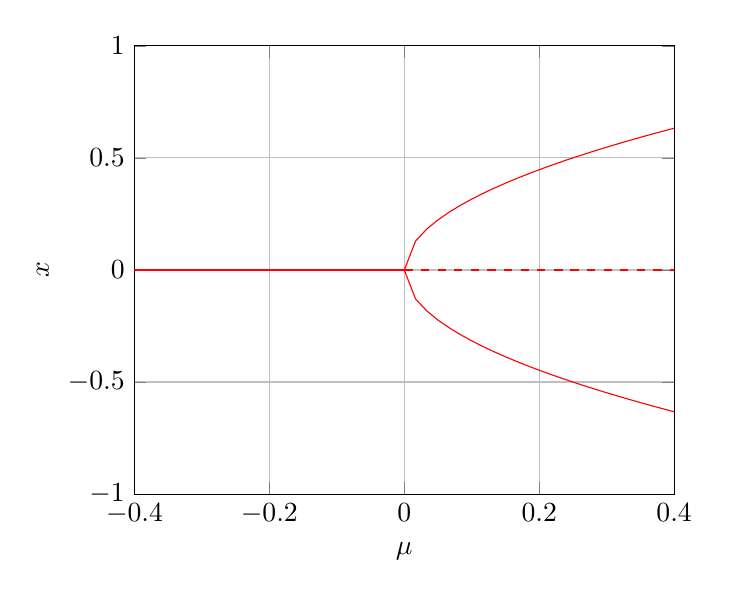
\begin{tikzpicture}[domain=-0.4:.4]
\begin{axis} [
    no markers, grid,
    domain=0:2,
    xmax=0.4, ymax=1,
    xmin=-0.4, ymin=-1,
    xlabel={$\mu$},
    ylabel={$x$}
    ]
\addplot +[red,domain=0:.4] plot (\x,{sqrt(\x)});
\addplot +[red,domain=0:.4] plot (\x,{-sqrt(\x)});
\addplot +[red,domain=-0.4:0] plot (\x,0);
\addplot +[red,dashed,domain=0:0.4] plot (\x,0);
\end{axis}
\end{tikzpicture}
\caption{Supercritical case}
\end{figure}


\subsubsection{Subcritical Pitchfork Bifurcations}
Basically reverse the stabilities of the supercritical pitchfork bifurcation. \\
E.x 
\[\dot{x} = f(x:\mu) = \mu x + x^3\]
Fixed points 
\[\mu x + x^3 = 0 \implies x_* = 0 , \pm \sqrt{-\mu}\]
So the second 2 fixed points will only exist for $\mu < 0$.
Stability:
\[f'(x) = \mu + 3x^2\]
For $x= 0$, $f'(x) = \mu$, $x=\pm\mu$, $f(x) = -2\mu$ .
So the fixed point, $x_*=0$,  is stable for $\mu <0$ and unstable for $\mu >0$.
For $x^* = \pm \sqrt{-\mu}$ it is unstable $\mu <0$ and doesn't exist for $\mu >0$.

Given an initial value of $\mu$ we know that in the long term we can tell what the system will do. e.g. if we choose $\mu = -1$. And the initial value of $x > \sqrt{-\mu}$. Since this lies above the fixed point, we expect the system to blow up to positive infinity. if $\mu > 0$, $x$ will tend to $\pm \infty$ depending on the sign of the initial $x$.

We say that the cubic term is destabilising

Back to the $\tanh x$ example. The taylor series ends up as
\[\tanh x = x - \frac13 x^3 + \frac2{15} x^5 - \frac{17}{315} x^7 + \mathcal{O}(x^9)\]
For $|x| < \frac{\pi}{2}$.
So we can (very roughly) approximate this by saying $\tanh x \approx x$ (for very small $x$). Or by saying
$\tanh x \approx x - \frac13 x^3$ (for slightly larger $x$). and then we can keep doing this as we want to bring $|x|$ closer to $\pi/2$.

The reasoning we are covering this is we can approximate solutions to
\[\dot{x} = \mu x - \tanh x\]
for small $x$ by approximating with:
\[\dot{x} \approx \mu x - (x - \frac13 x^3) \implies \dot{x} \approx \lambda x + \frac13 x^3\]
$\lambda := \mu -1$. This is the form of a subcritical bifurcation. So we know what will happen with the fixed points. 

Note that this will ONLY hold for small $|x|$. So we can't say that $x_*$ becomes unboundedly large under the same circumstances as before.

So if we then use the next larger term from the $\tanh x$ approximation, we can repeat the analysis and see how it changes the fixed points.
Remember that our approximation will completely stop holding for $|x| > \pi/2$

If out approximation maintains $|x| < \pi /2$ then the approximation is (relatively) valid.


We showed that by increasing $\mu$ or decreasing $\mu$ will have different outcomes for the path taken by $x$. This lack of reversibility is known as hysteresis. I.e. hysteresis is a lack of reversibility as a parameter is varied.



The region where the lack of reversibility occurs is known as a hysteresis loop. They are always one directional (in this example it was an anticlockwise loop). When you sketch the loop you must show direction


Spruce budworm model
\[\frac{dN}{dt} = RN(1 - \frac{N}{K}) - p(N), \quad N(0) = N_0\]
Where $N(t)$ is the budworm population at $t$. And we assume it is logistic with a linear birth rate $R$, and carrying capacity $K$.

The $p(N)$ term is predation:
\[p(N) = \frac{BN^2}{A^2 + N^2}\]
For small $N = \epsilon$ we get
\[p(\epsilon) = \frac{B\epsilon^2}{A^2} \to 0\]
For large $N$
\[p(N) = B, \quad N\gg A\]

For $N \lessapprox  A$, $p$ is small, and so predation is low (refuge state). For $N \gtrapprox  A$, predation is large so predation is high ().



Firstly we want to get the non-dimensional form
\[\frac{d\hat{N}}{d\hat{t}} = r\hat{N} \left(1- \hat{N}/k\right) - \frac{\hat{N}^2}{1+\hat{N}^2}\]
And $\hat{N}(0) = \hat{N}_0$
Where
\[k = \frac KA,\ r = \frac{AR}{B},\ \hat{N} = \frac NA,\ \hat{t} = \frac{Bt}{A},\ \hat{N}_0 = \frac{N_0}A\]
For notational convenience let $x := \hat{N}$ 
\[f(x:r,k) = rx (1-x/k) - \frac{x^2}{1+x^2}\]


So we have 2 parameters now. So for the analysis of bifurcations we have more possibilities!

We want to know 
\begin{enumerate}
    \item For which values of $r,k$ will the budworm population be under control?
    \item For which values of $r,k$ will the budworm population outbreak?
\end{enumerate}
What do we mean by outbreak? The budworm population suddenly jumps from low to high as $r,k$ vary.
Similarly, what do we consider a low population or a high population? 
Define $x\lessapprox 1$ to be a low population and $x \gg 1$ to be a high population.

To play around with analysis:
First we could try setting one parameter constant, and vary the other (and then swap)
By fixing $k$ and varying $r$ ew can see that we have an unstable fixed point at $x=0$ always, and a stable fixed point near $x =rk$, and that there is some variation of the fixed points in the middle.

% \begin{figure}
%     \centering
%     \begin{tikzpicture}
%     \begin{axis}
%     [
%     no markers, grid,
%     domain=0:3.5,    
%     xmax=3.5, ymax=.1,
%     xmin=0, ymin=-.1,
%     xlabel={$\mu$},
%     ylabel={$x$}
% ]
%     \addplot+[red] plot (\x,{0.622*\x*(1-\x/6) - \x^2/(1+\x^2)});
%     \end{axis}
%     \end{tikzpicture}
%     \caption{Caption}
%     \label{fig:my_label}
% \end{figure}

We have a region called a bistable interval, since here are 2 stable intervals in that interval. This will give us a hysteresis loop.




Recap
\[\dot x = f(x:r,k) = rx\left(1-\frac xk\right) - \frac{x^2}{1+x^2}\]
Since we are studying an outbreak, we want to look at jumps based on variations of parameters. Where a jump is $x\approx 1$ jumping to $x\gg 1$

Initially fix one of the parameters and then vary the other.

The bistable interval has 2 saddle-node bifurcations.


The lower stable branch is a refuge state, whereas the jump at after the unstable branch is an outbreak.

Should relate this to the dimensional model. Recall
\[r = \frac{AR}{B},\quad k=\frac KA = 6\]


So if we increase $R$ (increased birth rate) or decrease $B$ (amount of predation), or increase $A$ while decreasing $K$ to keep $k$ fixed. Then we can cause an outbreak


If we want to try varying both parameters
Go back to the initial problem

\begin{align*}
    f(x:r,k) = rx\left(1-\frac xk\right) - \frac{x^2}{1+x^2}\\
    x\{r\left(1-\frac xk\right) - \frac{x}{1+x^2}\}
\end{align*}
So we know $x^* =0 $ is a fixed point. 

Note that for small $x$,
\[f(x:r,k) \sim rx \implies f_x \sim r > 0\]
So $x^* = 0$ is unstable since $f_x > 0$.
The other fixed points are given by
\begin{align*}
    r\left(1-\frac xk\right) &= \frac{x}{1+x^2} \\
    S(x:r,k) &= C(x)
\end{align*}
Note that we have a simple function containing parameters, and a complicated function with no parameters. Plot these and use the same logic as in the tute


\begin{figure}[h]
\centering
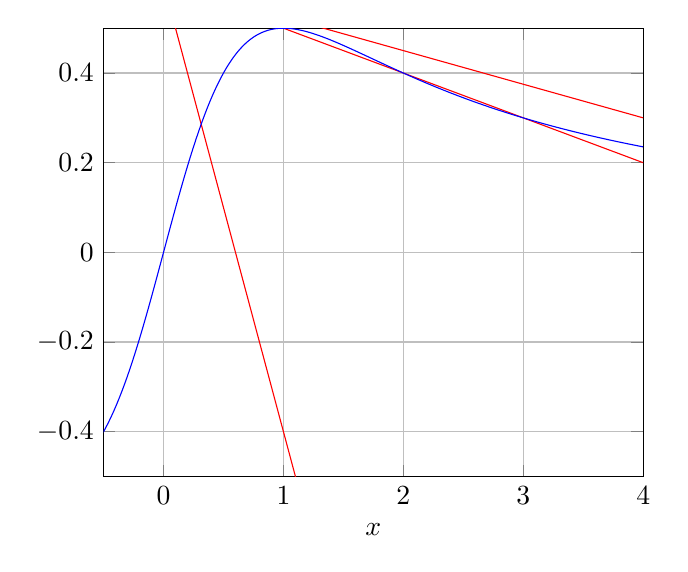
\begin{tikzpicture}[domain=-0.4:.4]
\begin{axis} [
    no markers, grid,
    domain=-1:5,
    xmax=4, ymax=0.5,
    xmin=-0.5, ymin=-0.5,
    xlabel={$x$},
    ]
\addplot +[red] plot (\x,{0.6*(1-\x/0.6)});
\addplot +[red] plot (\x,{0.6*(1-\x/6)});
\addplot +[red] plot (\x,{0.6*(1-\x/8)});
\addplot +[blue, samples=500] plot (\x,{\x/(1+\x^2)});
%\addplot +[red,dashed,domain=0:0.4] plot (\x,0);
\end{axis}
\end{tikzpicture}
\caption{Varying k for the two functions, blue is $C(x)$, red are the $S(x:r,k)$}
\end{figure}

Note that $f=xg \implies f_x = g+xg_x$. Since we want the fixed point at $g=0$ we can cross out the $g$ term in $f_x$.
\begin{align*}
    f_x = 0\\
    &\Leftrightarrow g + xg_x = 0\\
    &\Leftrightarrow g_x = 0\\
    &\Leftrightarrow (S-C)_x= 0\\
    &\Leftrightarrow S_x=C_x\\
    \dd{r\left(1-\frac xk\right) }x &= \dd{\frac{x}{1+x^2}}x\\
    -r/k &= \frac{(1+x^2) - 2x^2}{(1+x^2)^2} = \frac{1-x^2}{(1+x^2)^2}\\
    r &= \frac{k(x^2-1)}{(1+x^2)^2}\\
\end{align*}
Now we have to get the fixed point
\begin{align*}
    r(1-\frac xk) = \frac{x}{1+x^2}\\
    \frac{k(x^2-1)}{(1+x^2)^2} (1-\frac xk) = \frac{x}{1+x^2}
    \frac{k(x^2-1)}{1+x^2} (1-\frac xk) = x\\
     k-x = \frac{x(1+x^2)}{x^2-1}\\
     k = \frac{x(1+x^2)}{x^2-1} +x\\
     k = \frac{x(1+x^2) + x(1+x^2)}{x^2-1}\\
     k = \frac{x(x^2-1) + x(1+x^2)}{x^2-1}\\
     k = \frac{2x^3}{x^2-1}
\end{align*}
Substituting into the equation for $r$:

\begin{align*}
    r &= \frac{k(x^2-1)}{(1+x^2)^2}\\
    &=\frac{2x^3}{x^2-1}\times \frac{(x^2-1)}{(1+x^2)^2}\\
    r&=\frac{2x^3}{(1+x^2)^2}
\end{align*}
So the expressions for $r$ and $k$ are the bifurcation curves.

Since $k >0$ we must have $x > 1$. So bifurcations only occur for $x >1$.
Bifurcations will only occur when the bifurcation curves cross.


\begin{figure}[h]
\centering
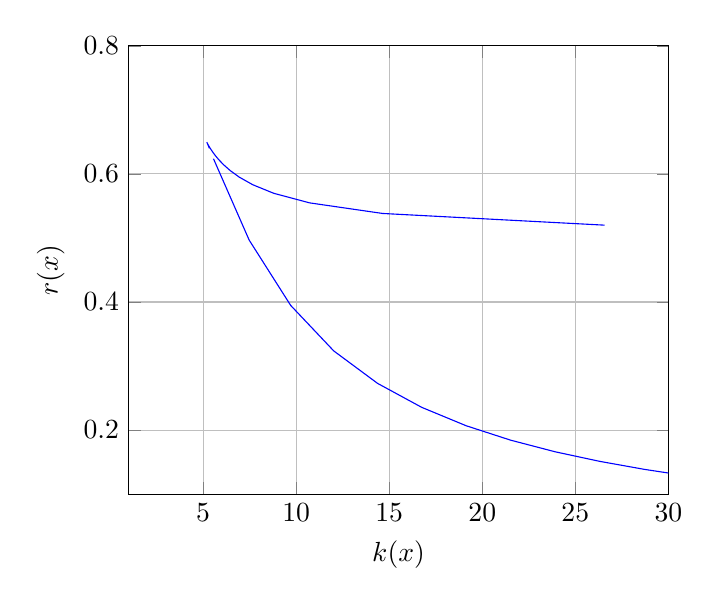
\begin{tikzpicture}
\begin{axis} [
    no markers, grid,
    xmax=30, ymax=0.8,
    xmin=1, ymin=0.1,
    xlabel={$k(x)$},
    ylabel={$r(x)$},
    ]
\addplot +[blue,domain=1:2] plot ({(2*\x^3)/(\x^2-1)},{(2*\x^3)/((1+\x^2)^2)});
\addplot +[blue,domain=1:30] plot ({(2*\x^3)/(\x^2-1)},{(2*\x^3)/((1+\x^2)^2)});
\end{axis}
\end{tikzpicture}
\caption{Bifurcation curves $k(x), r(x)$}
\end{figure}

% \begin{figure}
%     \centering
%     \begin{tikzpicture}
%     \begin{axis}[
%     no markers, grid,
%     xmax=3, ymax=6,
%     xmin=0, ymin=0,
%     ]
%     %\addplot3[surf] {x/((1+x^2)*(1-y)))};
%     \end{axis}
%     \end{tikzpicture}
%     \caption{Caption}
%     \label{fig:my_label}
% \end{figure}


Bifurcation diagram is now $x^*$ against $(k,r)$. Fixed points 
\[r(1-\frac xk) - \frac{x}{1+x^2} = 0\]
Introduce $y=x/k > 0$ as $x,k>0$. Then
\[r = \frac{x}{(1+x^2)(1-y)}\]


In practical terms our analysis says that an outbreak of the pest corresponds to a small change in the environment (slight change in parameter values), which can result in the population jumping from the lower stable branch to the upper (outbreak). Refuge happens with the opposite


\section{2D Autonomous Systems}
So now we will consider the fixed points, stabilities and bifurcations in two-dimensional (second-order) ODE models, expressed as systems of two first-order ODEs with two unknown functions. 

\subsection{Qualitative Analysis of 2D Systems}
Consider
\[\frac{dx}{dt}= f(x,y), \quad \frac{dy}{dt} = g(x,y)\]
Or in shorthand
\[\dot{\vec x} = \vec f(\vec x)\]
Where $\vec x = (x,y)$ and $\vec f(\vec x) = \left(f,g\right)$

And recall this is autonomous since $f,g$ do not explicitly depend on time.


The goal is to be able to perform analysis including:
\begin{enumerate}
    \item Phase \textit{plane} analysis
    \item Sketching \textit{phase portraits}
    \item Identifying steady states and \textit{nullclines}
    \item Determining stability
    \item Identifying \textit{periodic orbits} and \textit{limit cycles}
    \item Identifying bifurcations
\end{enumerate}

Definitions
\begin{itemize}
    \item \textbf{Phase plane:} $xy$-space
    \item \textbf{Vector Field:} phase plane containing vectors $\vec f(\vec x)$
    \item \textbf{Direction field:} vector field in which all vectors have same length
    \item \textbf{Trajectory/orbit:} solution curve $\vec x(t)$ (i.e. one path from the vector field)
    \item \textbf{Phase portrait:} phase plane with `typical' solutions shown (i.e. realistic trajectories)
\end{itemize}
Note that we're working with $(x(t),y(t))$ as parametric equations.

To help with phase portraits, define \textbf{Nullclines}:

The $x$-\textbf{nullcline} is $n_x=\{(x,y) : f(x,y) = 0\}$.\\
The $y$-\textbf{nullcline} is $n_y=\{(x,y) : g(x,y) = 0\}$.

On $n_x$, vectors $\vec f$ are vertical. On $n_y$, vectors $\vec f$ are horizontal (since we have ignored $g,f$ respectively.

Steady states/fixed points/equilibria are now points $(x,y) = (x^*,y^*)$ or $\vec x = \vec x^*$ such that
\[f(x^*,y^*) = g(x^*,y^*) = 0, \quad or, \quad  \vec f (\vec x^*) = \vec 0\]

They occur where $x$ and $y$ nullclines (i.e. $\eta_x,\eta_y$) intersect.

\subsection{Linear Systems}
The archetypical linear system:
\begin{align*}
    \dot x &= \alpha x + \beta y\\
    \dot y &= \gamma y + \delta x
\end{align*}

Or in vector notation
\[\vec{\dot x} = A\vec x \implies 
\begin{pmatrix}\dot x\\\dot y\end{pmatrix} =
\begin{pmatrix}\alpha & \beta \\\delta &\gamma \end{pmatrix}
\begin{pmatrix}x\\y\end{pmatrix}
\]

Solutions of this system have form:
\[\vec x = c_1 \vec v_1 e^{\lambda_1 t} + c_2 \vec v_2 e^{\lambda_2 t}\]
Where $\lambda_i$, $v_i$ are the eigenvalues and eigenvectors of $A$ respectively, $c_i$ are constants which depend on the ICs.

We assume that eigenvalue and eigenvector pairs exist here.

\subsubsection{Real Eigenvalues}
Consider the degenerate case where we set $\beta = \delta = 0$:
\begin{align*}
    \dot x &= \alpha x\\
    \dot y &= \gamma y
\end{align*}

The x-nullcline: setting $\alpha x = 0$, which is through $x=0$. (if $\alpha\neq 0$).\\
The y-nullcline: setting $\gamma y = 0$, which is through $y=0$.

So the the steady state is $\vec x^* = (0,0)$

The general form of the solution to this system is
\begin{align*}
    x(t) &= x(0) e^{\alpha t}\\
    y(t) &= y(0) e^{\gamma t}
\end{align*}
So $\lambda_1 = \alpha$, $v_1 = (1,0)^T$ and $\lambda_2 = \gamma$, $v_2 = (0,1)^T$


What happens when we change $\alpha$, $\gamma$?
\begin{enumerate}
    \item $\alpha,\gamma >0$ we see that the steady state is unstable - a kick in any direction will be \textbf{repelled} from the steady state. We call this a source. I.e. everything comes out of the fixed point
    \item $\alpha,\gamma <0$ the steady state is stable- any initial value will be absorbed in the steady state. We call this a sink.
    \item $\alpha > 0, \gamma <0$ the steady state is unstable for $x\neq 0$. We call this a saddle. The $y$ nullcline causes the instability.
    \item $\alpha <0, \gamma >0$ will be the same as (3) except swapping $x$, and $y$.
\end{enumerate}

\subsubsection{Complex Eigenvalues}
Now if we instead set $\gamma = -\beta$ and $\delta = \alpha$

\[\vec{\dot x} = A\vec x \implies 
\begin{pmatrix}\dot x\\\dot y\end{pmatrix} =
\begin{pmatrix}\alpha & \beta \\-\beta &\alpha \end{pmatrix}
\begin{pmatrix}x\\y\end{pmatrix}
\]
And assume $\beta \neq 0$.
The $x$-nullcline is 
\[\alpha x + \beta y = 0 \implies y = -\alpha x/\beta\]
The $y$-nullcline is
\[-\beta x + \alpha y = 0 \implies y = \beta x/\alpha\]
Where the fixed point is $\vec x^* = (0,0)$.

Eigenvalues and eigenvectors:
\[\lambda_1 = \alpha + i\beta, \quad \lambda_2 = \alpha - i\beta\]
\[\vec v_1 = (1,i), \quad \vec v_2 = (1,-i)\]

I should probably relearn how to calculate these.

So the general solution is

\begin{align*}
    \vec x(t) &= c_1 e^{\lambda_1 t} \vec v_1 + c_2 e^{\lambda_2 t} \vec v_2\\
    &= c_3 e^{\alpha t} \begin{pmatrix}
    \cos(\beta t + \phi)\\ -\sin (\beta t + \phi)
    \end{pmatrix}
\end{align*}
We did this since the original problem didn't have complex numbers. $\phi$ is introduced as the phase. So now our constants are $c_3,\phi$ rather than $c_1,c_2$.

Parameter cases:
\begin{enumerate}
    \item $\alpha = 0$. This gives solution
    \[\vec x = c_3 \begin{pmatrix}\cos(\beta t + \phi)\\ -\sin (\beta t + \phi) \end{pmatrix}\]
    This is a rotating field with only circular solutions - which are known as closed trajectories. What is the stability of the steady state for this case?

    \item $\alpha > 0$

    \item $\alpha < 0$ This gives a spiral sink - this is also known as a stable spiral. So it spirals towards the steady state at $0$. This is stable.

\end{enumerate}


\subsubsection{General Linear system}
now the general system
\[\frac{d}{dt} \begin{pmatrix}
    x\\y
\end{pmatrix} = \begin{pmatrix}
a&b\\c&d
\end{pmatrix} \begin{pmatrix}
    x\\y
\end{pmatrix}\]

Assuming $\det A\neq 0$ then we can diagonalise $A$ as
\[A = PBP^{-1}\]
Where $B = diag\{\lambda_1,\lambda_2\}$ and $P = [\vec v_1,\vec v_2]$ 

This gives
\begin{align*}
    \dot x = Ax = PBP^{-1} x\\
    \implies P^{-1} \dot x = BP^{-1} x\\
    \frac{d}{dt}(P^{-1} x) = B (P^{-1} x)\\
    \dot w = B w
\end{align*}
Where $\vec w = P^{-1} \vec x$, or $\vec x = P\vec w$. I.e. the derivative of $\vec w$ is just a linear transformation of $\vec w$.
Note that $B$ is diagonal. We know how diagonal systems behave (look back to the example). 

\begin{enumerate}
    \item $\lambda_1,\lambda_2 \in \mathbb{R}$ gives source,sink or saddle
    \item $\lambda_1 = \bar{\lambda_2} \in \mathbb{C}$ gives spiral or center
\end{enumerate}

We will find that $\vec x$ has the same \textbf{type} of behaviour as $\vec w$.


\subsubsection{Asymptotic Stability}
Solutions converge to the steady state when both eigenvalues are $\lambda_1,\lambda_2 < 0$ (if they're real). The origin becomes a stable node.
Or when the real \textbf{parts} of the eigenvalues are negative $\alpha <0$. Then we get a stable spiral.

When solutions converge to the steady state, then we say that the steady state is \textit{asymptotically stable}


Theorem:
For a two-dimensional linear system $\dot{\mathbf{x}}= A \mathbf{x}$, the following are equivalent:

\begin{enumerate}
    \item The equilibrium $(0,0)$ is asymptotically stable
    \item all eigenvalues of $A$ have negative real part
    \item $\det A> 0$ and $tr A < 0$
\end{enumerate}

Proof:
By definition $(1) \Leftrightarrow (2)$.
For $(3)$, consider the characteristic equation of $A$:
\begin{align*}
    (a-\lambda) (d-\lambda) - bc = 0\\
    ad - (a+d)\lambda + \lambda ^2  - bc =0\\
    \lambda ^2  - (a+d)\lambda +(ad- bc) =0\\
\end{align*}
Note that $(a+d) = tr A$, and $(ad-bc) = \det A$

\[\lambda = \frac12 trA \pm \sqrt{(tr A)^2 - 4\det A}\]
For the complex $\lambda$ case, we require the real part to be negative: $tr A <0$.

For real $\lambda$, we require the discriminant to be positive. For asymptotic stability we need the real part of both to be $0$. So we require $\det A > 0$.


Hand wavey argument but we'll leave it as that


Basically we just need to calculate the trace and the determinant of $A$ to determine whether or not the system is asymptotically stable.
\begin{itemize}
    \item $\det A > 0$
    \begin{itemize}
         \item $tr A > 0$ Unstable region:
         \begin{itemize}
             \item $det A > \frac14 (tr A)^2$ unstable spiral
             \item $det A < \frac14 (tr A)^2$ unstable node
         \end{itemize}
         \item $tr A < 0$ Asymptotically stable region.
         \begin{itemize}
             \item $det A > \frac14 (tr A)^2$ stable spiral
             \item $det A < \frac14 (tr A)^2$ stable node
         \end{itemize}
         \item $tr A = 0$ centre behaviour
     \end{itemize} 
    \item $\det A < 0$ not stable.
\end{itemize}





\subsection{Nonlinear Systems and Linearisation}
\subsubsection{General nonlinear system}
Consider the two dimensional nonlinear system:
\begin{align*}
    \dot x = f(x,y)\\
    \dot y = g(x,y)
\end{align*}
Where we will assume  $f,g$ are continuously differentiable functions.
Each point $\mathbf{x}^* = (x^*,y^*)$ satisfying $f(x^*,y^*) = g(x^*,y^*) = 0$ is a fixed point/equilibrium/steady state.

\textbf{Definitions}
\begin{enumerate}
\item A steady state $\mathbf{x}^*$ is stable if a solution which starts nearby stays nearby
\item A steady state $\mathbf{x}^*$ is unstable if it is not stable.
\item A steady state $\mathbf{x}^*$ is asymptotically stable if $\mathbf{x}^*$ is stable, and all solutions near $\mathbf{x}^*$ converge to $\mathbf{x}^*$.
\end{enumerate} 
We can determine stability through linearisation

\subsubsection{Linearisation}
Suppose we are close to a steady state $\mathbf{x} = \mathbf{x^*}$ then
\[\mathbf{x}(t) = \mathbf{x^*} + \mathbf{w}(t), \quad \mathbf{w}(t) = \begin{pmatrix}
w(t)\\z(t)
\end{pmatrix}\]
And $||\mathbf{w}\ll 1$


Take a taylor series (we will have to do this in x and y). We will only do this to the linear terms
\begin{align*}
    f(x,y) = f(x^*+w,y^*+z) &= f(x^*,y^*) + w f_x(x^*,y^*) + zf_y(x^*,y^*) + \ldots\\
    &= w f_x(x^*,y^*) + zf_y(x^*,y^*) + \ldots\\
    g(x,y) &= wg_x(x^*,y^*) + zg_y(x^*,y^*) + \ldots
\end{align*}

So we get
\[\mathbf{f}(\mathbf{x}) = J(\mathbf{x}^*)\mathbf{w} + \ldots\]
Where 
\[J(\mathbf{x}) = \begin{pmatrix}
    f_x(\mathbf{x})&f_y(\mathbf{x})\\
    g_x(\mathbf{x})&g_y(\mathbf{x})\\
\end{pmatrix}\]
Is the Jacobian

Hence close to $\mathbf{x}^*$
\[\dot x = \dd{}t(\mathbf{x}^* + \mathbf{w}) \implies \dot{\mathbf{w}} \approx J(\mathbf{x}^*)\mathbf{w}\]
This is a linear system. Which can be solved easily.


\textbf{Definition}:
The steady state $\mathbf{x}^*$ is called \textit{hyperbolic} if \textbf{all} eigenvalues of the Jacobian $J(x^*,y^*)$ have non-zero real part

\textbf{Theorem}: Hartman-Grobman Theorem\\
Assume that $\mathbf{x}^*$ is a \textit{hyperbolic equilibrium}. Then, in a small neighbourhood of $\mathbf{x}^*$, the phase portrait of the nonlinear system
\begin{align*}
    \dot x = f(x,y)\\
    \dot y = g(x,y)
\end{align*}
Is equivalent to that of the linearised system.

I.e. near a \textit{hyperbolic equilibrium}, $\mathbf{x^*}$, we can use the linearised problem.
\[\dot{\mathbf{x}} = A \mathbf{x} \]
Where $A = J(\mathbf{x}^*)$

So if we calculate the trace and determinant of $A$ we know about the stability of the state and its type.

\[\lambda_\pm = \frac12 \{tr A \pm \sqrt{(tr A)^2 - 4\det A}\} \]
We require the real part of BOTH $\lambda$s to be nonzero. 
So we \textbf{cant} have:
\begin{itemize}
    \item  $tr A = 0$  with $\det A >0$
    \item $\det A = 0$ 
\end{itemize}


\subsection{Application to models}
\subsubsection{Interaction model for 2 populations}
Consider 2 interacting populations. Each has exponential growth with some interaction term proportional to both of them
\begin{align*}
    \frac{dx}{dt} &= \alpha x + \beta xy\\
    \frac{dy}{dt} &= \gamma y + \delta xy
\end{align*}


This is clearly \textit{not} a linear model.

\begin{table}
\centering
     \begin{tabular}{c|c|c|c|l}  
        $\alpha$ & $\beta$ & $\gamma$ & $\delta$ & \\
        \hline
        +&+&+&-&Predator$(x)$, prey$(y)$ models\\
        +&+&-&-&Predator$(x)$, prey$(y)$ models\\
        -&+&+&-&Predator$(x)$, prey$(y)$ models\\
        -&+&-&-&Predator$(x)$, prey$(y)$ models\\
        \hline
        +&-&+&+&Predator$(y)$, prey$(x)$ models\\
        +&-&-&+&Predator$(y)$, prey$(x)$ models\\
        -&-&+&+&Predator$(y)$, prey$(x)$ models\\
        -&-&-&+&Predator$(y)$, prey$(x)$ models\\
        \hline
        +&+&+&+&Mutualism / symbiosis models\\
        +&+&-&+&Mutualism / symbiosis models\\
        -&+&+&+&Mutualism / symbiosis models\\
        -&+&-&+&Mutualism / symbiosis models\\
        \hline
        +&-&+&-&Competition Models\\
        +&-&-&-&Competition Models\\
        -&-&+&-&Competition Models\\
        -&-&-&-&Competition Models\\
     \end{tabular}
\end{table} 



Write
\[\begin{cases}
    f(x,y) = \alpha x + \beta xy\\
    g(x,y) = \gamma y + \delta xy
\end{cases}\]

Nullclines
\[\begin{cases}
    n_x : \alpha x + \beta xy = 0 &\implies x =0, y = -\alpha/\beta\\
    n_y : \gamma y + \delta xy = 0 &\implies y =0, x = -\delta/\gamma
\end{cases}\]

Note this is a population model, so we require ``biologically relevant solutions'' $x,y \geq 0$


\begin{figure}[h]
\centering
\begin{tikzpicture}
\begin{axis} [
    no markers,
    domain=0:1,
    xmax=1.2, ymax=1.2,
    xmin=-0, ymin=0.2,
    xlabel={$x$},
    ylabel={$y$}
    xticklabels{},yticklabels={},
    ]
\addplot +[green,domain=0:1] plot (\x,1);
\addplot +[red,domain=0:1] plot (\x,0);
\addplot +[green,domain=0:1] plot (0,\x);
\addplot +[red,domain=0:1] plot (1,\x);
\end{axis}
\end{tikzpicture}
\end{figure}
We only care about 2 intersections: $x,y = (0,0)$ and the top right intersection.

Calculate the jacobian:
(I HAVEN"T FINISHED THIS PART)
\[J(0,0) = \begin{pmatrix}
    f_x(0,0)& f_y(0,0)\\
    g_x(0,0)&g_y(0,0)
\end{pmatrix} = \begin{pmatrix}
    \alpha&0\\ 0&\gamma
\end{pmatrix}\]
Which has 
\[\begin{cases}
    trace = \alpha + \gamma\\
    det = \alpha\gamma
\end{cases}\]
Hence 
\[\begin{cases}
    \lambda_1 = \alpha \\
    \lambda_2 = \gamma
\end{cases}\]
$\lambda$'s are real. We don't know if its a source, sink or saddle until we know the signs of $\alpha,\gamma$.


For the second steady state:

\begin{align*}
    J(-\gamma/\delta, -\alpha/\beta) &= \begin{pmatrix}
        \alpha - \beta \alpha/\beta & -\beta \gamma/\delta\\
        -\delta \alpha/\beta & \gamma - \delta \gamma/\delta
    \end{pmatrix}\\
    &= \begin{pmatrix}
        0 & -\beta \gamma/\delta\\
        - \alpha \delta/\beta & 0 \\
    \end{pmatrix}\\
    &=: A
\end{align*}
We have
\[\begin{cases}
    tr A = 0\\
    \det A = - \alpha \gamma
\end{cases}\]
\begin{align*}
    \lambda_{\pm} &= \frac12\{trA \pm \sqrt{(tr(A))^2 - \frac14 \det A}\}\\
    &=\pm \sqrt{\det A}\\
    &= \pm \sqrt{\alpha \gamma}
\end{align*}
Which will be a centre if $\alpha\gamma < 0$ or a saddle if $\alpha\gamma >0$


\subsubsection{Lutka-Voltera predator-prey model:}
$\alpha <0$, $\beta > 0$, $\gamma > 0$ and $\delta < 0$.
From the table, $x$ is the predator while $y$ is the prey. Since $\alpha <0$ the predator while die out without prey, and $\gamma >0$ the prey will grow out of control without the predator.

At the steady state $P_1 = (0,0)$
\[\lambda = \begin{cases}\alpha < 0\\\gamma > 0\end{cases} \implies P_1 \text{ is a saddle}\]

At $P_2 = (-\gamma/\delta, -\alpha/\beta)$:
Is the steady state biologically relevant? $-\gamma/\delta > 0$ and $-\alpha/\beta >0$ so yes.

\[det A = -\alpha\gamma > 0\]
So $P_2$ is a centre (in the linearised problem)
And
\[\lambda_\pm = \pm i \sqrt{|\alpha \gamma|}\]
Which is purely imaginary. The real part is zero - so $P_2$ is not hyperbolic, and so the linearised problem cannot be used.


Instead write the system in a different form (it comes out as a separable ODE)
\begin{align*}
    \frac{dy}{dx} &= \frac{\frac{dy}{dt}}{\frac{dx}{dt}}\\
    \frac{dy}{dx} &= \frac{g}{f} \\
    \frac{dy}{dx} &= \frac{y(\gamma + \delta x)}{x(\alpha + \beta y)}\\
    \int \frac{\alpha + \beta y}y dy &= \int \frac{\gamma + \delta x}{x} dx\\
    \alpha \int \frac1y dy + \beta \int 1 dy &= \gamma \int \frac1x dx + \delta \int 1 dx\\
    \alpha \log y + \beta y &= \gamma \log x + \delta x + C\\
    &\text{let } \alpha = -1 = \delta,\quad \beta =1 =\gamma\\
    \log y + \log x &= - C + x + y\\
    xy &= e^{-C+x+y}\\
    \frac{e^{x+y}}{xy} &= B = e^{C}
\end{align*}
Where $B$ is determined by the initial conditions



This gives a nonlinear centre.
The corresponding solutions for $x(t)$ and $y(t)$ oscillate around the steady state.

\subsubsection{Mutualism model}
$\alpha <0$, $\beta>0$, $\gamma <0$, $\delta>0$
I.e. neither can survive alone.

At $P_1(0,0) $
\[\begin{cases}
    \lambda_1 = \alpha < 0\\
    \lambda_2 = \gamma <0
\end{cases}\]
Hence $P_1$ is a sink (stable node).


At $P_2$ check if it is biologically relevant: $-\gamma/\delta >0$ and $-\alpha/\beta > 0$ so it is!

$detA = -\alpha \gamma <0$ so $P_2$ is a saddle
\[\lambda_\pm = \pm \sqrt{\alpha \gamma}\]
Since $Re(\lambda_\pm) \neq 0$ the HG theorem applies (the linearised problem works here).


To sketch a phase portrait (by hand) start with the nullclines:
On $\eta_x$ where $y = -\alpha/\beta > 0$, 
\[g = \gamma y + \delta xy = -\alpha/\beta(\gamma + \delta x) \begin{cases}
    > 0 & \gamma+\delta x > 0 \implies x > -\gamma/\delta\\
    < 0 & \gamma+\delta x < 0 \implies x < - \gamma/\delta
\end{cases}\]
On $\eta_y$, where $x = -\gamma/\delta$
\[f = \alpha x + \beta xy = -\gamma/\delta(\alpha + \beta x) \begin{cases}
    > 0 & \alpha+\beta x > 0 \implies y > -\alpha/\beta\\
    < 0 & \alpha+\beta x < 0 \implies y < - \alpha/\beta
\end{cases}\]

The other piece of information we can use is the steady and unsteady directions from the saddle.
For $P_2$ we have
\[V_\pm = \begin{pmatrix}
    \pm 1\\1
\end{pmatrix}\]
Noting that $V_+$ will be the unstable direction: since $\lambda_+ > 0$ and $V_-$ will be stable since it is related to the negative eigenvalue



\subsubsection{Competition model}
$\alpha>0, \beta<0, \gamma<0, \delta<0$

At $P_1=(0,0)$
\[\begin{cases}
    \lambda_1 = \alpha > 0\\
    \lambda_2 = \gamma <0 
\end{cases}\implies P_1 \text{ is a saddle}\]

\[J(0,0) = \begin{pmatrix}
    \alpha&0\\0&\gamma
\end{pmatrix} \implies v_1 = \begin{pmatrix}
    1\\0
\end{pmatrix}, \quad v_2 =\begin{pmatrix}
    0\\1
\end{pmatrix}\]
Since its a diagonal matrix the eigenvectors are really simple.
Unstable direction is $v_1$, since $\lambda_1 = \alpha > 0$ and $\lambda_2 = \gamma < 0$ gives the stable $v_2$.

The second steady state $P_2 = (-\gamma/\delta, -\alpha/\beta)$ is it biologically relevant? 
\[-\alpha/\beta >0 ,\quad -\gamma/\delta < 0\]
So no this is not biologically relevant.





\subsection{The Kermack-McKendrick epidemic model}
Start with the $SIRS$ model. 
\begin{align*}
    \frac{dS}{dt} &=-\beta IS + \gamma R \\
    \frac{dI}{dt} &=\beta IS - \alpha I \\
    \frac{dR}{dt} &= \alpha I - \gamma R
\end{align*}

The model has units people per unit time. It contains a nonlinear term, $\beta IS$.

$\beta I > 0$ is the rate at which $S$ become $I$.

$\alpha > 0$ is the rate at which $I$ become $R$.

$\gamma > 0$ is the rate at which $R$ become $S$.

This is a $3D$ model. So lets make it $2D$.

First we will just consider the $SIR$ model, so $\gamma = 0$

We can drop $\frac{dR}{dt}$ since it now gives no information and isn't in the other equations. The $SIR$ model is the KM model. If we know $S(t)$ and $I(t)$ then we can find 
\[R(t) = N - S(t) - I(t)\]
Where $N$ is the fixed population size.

\begin{align*}
    \frac{dS}{dt} &=-\beta IS\\
    \frac{dI}{dt} &=\beta IS - \alpha I \\
\end{align*}

We won't bother non-dimensionalising because it makes life easier. This is effectively a predator prey model, where the prey is constant if there are no infected.


The $S$- nullcline $\beta IS = 0$, so either $I=0$ or $S=0$\\
The $I$- nullcline $\beta IS - \alpha I$ = 0. So either $I=0$ or $S = \alpha/\beta$


The steady states are along the $S$ axis. I.e. whenever $I=0$ we have a steady state. We will call this a \textbf{ray} of steady states.


The Jacobian:
\[J(S,I) = \begin{pmatrix}
    -\beta I & -\beta S\\ \beta I & \beta S - \alpha
\end{pmatrix}\]
Along the ray 
\[J(S^*,0) = \begin{pmatrix}
    0& -\beta S_*\\
    0 & \beta S_* - \alpha
\end{pmatrix} = A\]

\[\begin{cases}
    trA &= \beta S_* - \alpha\\
    \det A &= 0
\end{cases}\]

Hence $\lambda_1 = 0$ and $\lambda_2 = \beta S_* - \alpha$

Thus all the steady states are non-hyperbolic so we cannot use the linearised problem.
Note that $\lambda_2 < 0 $ if $S_* < \alpha/\beta$

\begin{align*}
    f=  -\beta IS\\
    g = BI(S-\frac{\alpha}\beta)
\end{align*}
So $f$ is everywhere pointing left
$g$ points down for $S < \frac \alpha \beta$ and points up for $S > \frac \alpha \beta$

Hence $S < \frac \alpha \beta$ with $I=0$ is a steady state, and $S > \frac \alpha \beta$ with $I=0$ is an unsteady state.
To really construct the phase portrait use the trick we used for the predator prey model:
\[\frac{dI}{dS} = \frac{\dot{I}}{\dot{S}} = \frac{I(\beta S - \alpha)}{-\beta IS} = -1 + \frac{\alpha}{\beta S}\]
Hence
\[I = -S + \frac{\alpha}\beta \log S + C\]
Where
\[C = I_0 + S_0 - \frac{\alpha}\beta \log S_0\]
Where $I_0 = I(0)$ and $S_0 = S(0)$. 

So we can write $I$ in terms of $S$.
\[I(S) = I_0 + S_0 - S + \frac{\alpha}{\beta} \log \frac{S}{S_0}\]
And then we can plot!


\subsection{Big Recap}
2D Autonomous Systems.
\begin{align*}
    \dot{x} = f(x,y)\\
    \dot{y} = g(x,y)
\end{align*}

or alternatively
\[\dot{\mathbf{x}} = f(\mathbf{x})\]

Phase portraits require: 
\begin{itemize}
    \item nullclines 
    \begin{itemize}
         \item $x$ nullcline, $\eta_x$ where $f(x,y) = 0$
         \item $y$ nullcline, $\eta_y$ where $g(x,y) = 0$
     \end{itemize} 
     \item Steady states - intersection of an $x$ and a $y$ nullcline.
     \item Vector field
     \item Trajectories/orbits
\end{itemize}

\textbf{Linear systems:} unique fixed point at origin.
\begin{align*}
    \dot{x} = \alpha x + \beta y\\
    \dot{y} = \gamma y + \delta x
\end{align*}
Solutions have form
\[\mathbf{x} = c_1 \mathbf{v}_1 e^{\lambda_1 t} + c_2 \mathbf{v}_2 e^{\lambda_2 t}\]

They display one of the following behaviours:
\begin{itemize}
    \item Unstable behaviour (source or unstable node) 
    \item Stable behaviour (sink or stable node)
    \item Saddle behaviour
    \item Centre (closed orbits)
    \item Unstable spiral
    \item Stable spiral
\end{itemize}

The behaviour is determined by the trace and determinant of the matrix.


For non-linear systems
\begin{align*}
    \dot{x} = f(x,y)
    \dot{y} = g(x,y)\\
\end{align*}

HG theorem: near a hyperbolic steady state (linearised system only has non-zero eigenvalues), the linear system is equivalent to the linear system.



\subsection{Limit Cycles}
In 1D/scalar sstems, solutions either tend to fixed points or become unbounded.\\
In 2D autonomous systems, we can get periodic solutions (closed trajectories around center).

If we now consider
\begin{align*}
    \dot{r} = r(1-r^2)\\
    \dot{\theta} = 1
\end{align*}
In polar coords ($r,\theta$) (convert back with $x = r\cos\theta, y= r\sin \theta$)

For the $r$ equation, the steady states are $r_* = 0,\pm1 $
And we get $r_* = 0$ is unstable, $r_* = 1$ is stable.
In cartesian coordinates this will move us into the fixed circle $r=1$. I.e. the circle $x^2 + y^2 = 1$

If we solve the second equation, we get:
\[\theta = t + \theta_0\]
So $\theta$ changes continuously.

So we expect to spiral until we reach the unit circle (whether we come from inside or outside)
I.e. $r_* =0$ is an unstable fixed point (an unstable spiral), 
The circle $r_*=1$ is known as a \textbf{limit cycle}. It is an isolated closed orbit.


If we plot this for $x$ and $t$, we find all solutions tend towards a single periodic solution. This is the sign of a limit cycle.


\subsection{Bifurcations in 2D systems}
We already did this for $1D$. Same thing occurs in 2D: fixed points can be created or destroyed or destabilised with parameter changes. The difference is that closed orbits can do the same thing as fixed points. In 2D we say a bifurcation has occurred if the phase portait changes its topological structure as a parameter is varied. 

\subsubsection{Saddle-node, transcritical and pitchfork bifurcations}
The bifurcations of all 1D fixed points have 2D analogs. We find that one of the two dimensions will do what we saw in 1D, while in the second dimension there will simply by attraction or repulsion.

Example
\begin{align*}
    \dot x &= \mu - x^2 = f(x,y)\\
    \dot y &= - y = g(x,y)
\end{align*}
These are decoupled, so they will be easy to work with, and $\mu$ only appears in the $x$ equation.

The $x$ equation is the standard form for a saddle node bifurcation. $\mu > 0$ gives 2 fixed points ($x_*=\pm\sqrt{\mu}$, positive is stable, negative is unstable), $\mu = 0$ gives 1 fixed point and $\mu <0$ gives 0 fixed points.

The $y$ equation has the fixed point $y_*=0$, which will be stable.

Thus in the 2D system, for $\mu>0$ there are two fixed points $\vec{x_*} = \left(-\sqrt{\mu},0\right)$ and $\left(\sqrt{\mu},0\right)$. The positive one is a sink, the negative one is a saddle.

for $\mu <0$ there are no fixed points.

For $\mu=0$ the fixed point is non-hyperbolic interestingly enough.


We won't bother with the other canonical examples because they're the same analysis as this.


\subsubsection{Hopf Bifurcation}
Consider the system
\begin{align*}
    \dot x = -y + x(\mu - x^2 - y^2)\\
    \dot y = x + y(\mu-x^2-y^2)
\end{align*}
With $\mu \in \mathbb{R}$

We can rewrite this system in polar coordinates:
\begin{align*}
    \dot r &= r(\mu - r^2)\\
    \dot\theta &= 1
\end{align*}
Earlier, we saw that when $\mu=1$ we get a limit cycle. 

Recall $\dot r$ is the equation for a pitchfork bifurcation (in $\dot r$).
Fixed points $r_*=0,\sqrt{\mu}$ for $\mu > 0$ which is stable. Note that $r \geq0$ we cannot have $r<0$ due to the use of polar coordinates. 
$r_*=0$ is stable for $\mu <0$ and unstable for $\mu >0$


The Jacobian (in terms of $x,y$):

    
\[J = \begin{pmatrix}
    \mu -3x^2 - y^2 &-1 -2xy\\
    1-2xy & \mu - x^2 - 3y^2
\end{pmatrix}\]
At the fixed point $x_*=y_*=0$ 

\[J(0,0) = \begin{pmatrix}
    \mu&-1\\1&\mu
\end{pmatrix}\]
Referring to 3.2.2 this has eigenvalues $\mu\pm i$. Meaning the fixed point is a stable spiral for $\mu <0$, an unstable spiral for $\mu > 0$ and for $\mu =0$ it is non-hyperbolic.

At $r_* = \sqrt{\mu}$ ($\mu > 0$) we get the limit cycle behaviour with radius $\sqrt{\mu}$ so we get an `attracting limit cycle'

This is a \textbf{Hopf bifurcation}. I.e. the change of stability of a fixed point....







\section{Numerics!}
Easy shit!

We will look at numerical solutions of first order IVPs.
\[\frac{du}{dt} = f(u,t), \quad u(0) = u_0\]
However most concepts wlil extend to higher dimensions very straightforwardly.
We don't always need numerical solutions. We can get exact solutions thus far for:
\begin{itemize}
    \item Separable ODEs
    \item Linear ODEs
    \item Exact ODEs
    \item Homogeneous ODEs 
\end{itemize}

\textbf{Goals:}
\begin{enumerate}
    \item To understand the concept of a `well posed problem'
    \item How to apply the Picard-Lindelof theorem
    \item To be able to measure error, determine conditioning of a problem, and the statbility of a numerical algorithm
    \item To know some important finite difference numerical algorithms and how to choose them 
\end{enumerate}

\subsection{Existence and Uniqueness}
Canonical Example:

Consider the first order IVP of form:
\[\dot x = x^{1/3},\quad x(0) = 0\]
And assuming $x(t) \in \mathbb{R}$ for all $t\geq 0$.

Note this is a nonlinear ODE since we have a fractional power of the dependent variable.

Clearly the trivial solution works: $x(t) =0$

Note the ODE is separable:
\[x^{1/3} \dot x = 1 \implies \int x^{-1/3} dx = \int dt \implies \frac32 x^{2/3} = t+c\]
IC $x(0) = 0 \implies c=0$ 
\[\implies x(t) = \left(\frac{2t}{3}\right)^{3/2}\]
Hence
\[x(t) = \begin{cases}
    0& t < \hat c\\
    \left(\frac{2(t-\hat c)}{3}\right)^{3/2} & t\geq \hat c
\end{cases}\]
Is a solution also, for any $\hat c \geq 0$. This is a `family' of solutions. Also the square root has positive and negative branches.


If we attempted to obtain a numerical solution to this:

Using Euler's method:
\[\frac{dx}{dt} = \frac{x(t+h) - x(t)}{h}\]
\[\implies x_{n+1} = x_n + h x_n^{1/3}\]
Where $x_n \approx x(t_n)$ and $t_n = nh$.

Start with $x_0 = x(0) =0$
\[x_1 = x_0 + hx_0^{1/3} =0\]
And hence via iteration we get $x_n = 0$, i.e. the trivial solution.

\subsubsection{Well and Ill posed Problems}
For mathematical models of physical phenomena:
\begin{enumerate}
    \item A solution must exist
    \item The solution must be unique
    \item The solution's behaviour must change continuously with the initial conditions 
\end{enumerate}
If we have these 3 properties, the problem is well posed. Otherwise it is ill posed.

A well posed problem should give numerical solutions (it has a `good chance'), ill posed problems will not, and need to be reformulated.

\subsection{Existence and Uniqueness Theorem}
The Picard-Lindel\"of theorem 

Suppose $I = [t_-,t_+]$ is an interval in $t$ with $t_- \leq t_0 < t_+$ and $J=[u_-,u_+]$ is an interval in $u$ with $u_-<u_0<u_+$. If $f : I\times J \to \mathbb{R}$ is continuous on its domain, and Lipschitz continuous (shown below) on $J$, then there exists $\epsilon >0$ such that the IVP:
\begin{align*}
    \frac{du}{dt} =& f(t,u),\quad t\in [t_0,t_0+\epsilon]\\
    u(t_0) =& u_0
\end{align*}

Has a unique solution $u \in C^1 [t_0,t_0+\epsilon]$

Lipschitz continuity:

Let $J=[x_0,x_1]$ be an interval on the real line. We say $f: J\to \mathbb{R}$ is  \textbf{Lipschitz continuous} on $J$ if there exists $L>0$ such that
\[|f(x) - f(y)| \leq L|x-y|,\quad \text{for all } x,y\in J\]

Examples:

Show $f(x) = \sin x$ is Lipschitz continuous on $\mathbb{R}$. Let $x,y \in \mathbb{R}$, and assume $y < x$ (wlog)
\[\sin x - \sin y = (x - y)\cos c,\quad c \in (y,x)\]
Using the Mean Value Theorem (MVT)
So
\begin{align*}
    |f(x) - f(y)| &= |\sin x - \sin y|\\
    &=|(x - y)\cos c|\\
    &=|(x-y)||\cos c| \leq |x-y|
\end{align*}
Since $|\cos c| \leq 1 $ for all $c \in \mathbb{R}$

Thus $f(x) = \sin x$ is Lipschitz continuous, with $L=1$. 

We call the smallest possible value of $L$ the best Lipschitz constant.

We say $f=\sin x$ is globally Lipschitz continuous, since it is continuous over its entire domain, where not all functions will be.


Example 2:
\[g(x) = x^2\]
We could use the MVP as above, but theres a simpler approach:
\begin{align*}
    |g(x) - g(y)| &= |x^2 - y^2|\\
    &= |(x+y)(x-y)|\\
    &= |x+y||x-y|\\
\end{align*}
Using the fact that $|x+y| \leq |x|+|y|$ by the triangle inequality, consider $g$ on a bounded interval, say $J = [-1,1]$.


$g(x) = x^2$
Say we consider an odd interval $J$, e.g. $J=[-1,1]$, then $|x| + |y| \leq 2$
So that
\[|g(x)-g(y)| \leq 2 |x-y|\]
So $g$ is Lipschitz continous with best const $L=2$ on $J=[-1,1]$
However if $J$ is unbounded, e.g. $J =\mathbb{R}$. Then there doesn't exist an $L$.
But for any finite interval, then we have Lipschitz continuity.




If we have the ODE $\dot u = f(t,u)$ where $t \in I$ and $u \in J$, so we get $f:I\times J \to \mathbb{R}$. So we can plot this system in 3D as a surface plot. I.e. plotting $u,t,f$ (literally half of what im doing in my thesis...)











\subsection{Picard Iteration}



\subsection{Error, Conditioning and Stability}

\subsubsection{Error}

\subsubsection{Conditioning}

\subsubsection{Stability of algorithms}



\subsection{Finite Differences}










































\end{document}
